% !TeX spellcheck = en_GB
%\documentclass[twocolumn]{ceurart}
\documentclass{ceurart}
% version
\newcommand{\versionmajor}{0}
\newcommand{\versionminor}{1}
\newcommand{\versionpatch}{0}

\usepackage{ceur-article-template}

\begin{document}
	
\copyrightyear{2022}
\copyrightclause{Copyright for this paper by its authors. Use permitted under Creative Commons License Attribution 4.0 International (CC BY 4.0).}

\conference{$N^{st}$ Conference/Workshop ``Fancy Topic \& Buzzwords'' (FTB), Month 31--33, 20XX, Location, Country}

\title{Fancy title just to clickbait citations}
\tnotemark[1]
\tnotetext[1]{You can use this document as the template for preparing your publication. We recommend using the latest version of the ceurart style.}

\author[1]{Giovanni Ciatto}[orcid=0000-0002-1841-8996]\ead{giovanni.ciatto@unibo.it}
\cormark[1]
\fnmark[1]
\author[2]{Roberta Calegari}[orcid=0000-0003-3794-2942]\ead{roberta.calegari@unibo.it}
\fnmark[1]
\author[1]{Andrea Omicini}[orcid=0000-0002-6655-3869]\ead{andrea.omicini@unibo.it}
\fnmark[1]

\address[1]{Dipartimento di Informatica -- Scienza e Ingegneria (DISI), \textsc{Alma Mater Studiorum}---Università di Bologna, Italy}
\address[2]{Alma Mater Research Institute for Human-Centered Artificial Intelligence, \textsc{Alma Mater Studiorum}---Università di Bologna, Italy}

\cortext[1]{Corresponding author.}
\fntext[1]{These authors contributed equally.}

\begin{abstract}
    Catchy sentences here.
\end{abstract}

\begin{keywords}
    LaTeX class 
    \sep
    paper template 
    \sep
    paper formatting 
    \sep
    CEUR-WS
\end{keywords}

\maketitle

\section{Introduction}

Buzzords and stuff. 

\section{Background}

Citations, e.g. \cite{MR781536}

\section{Contribution}

\begin{figure}
    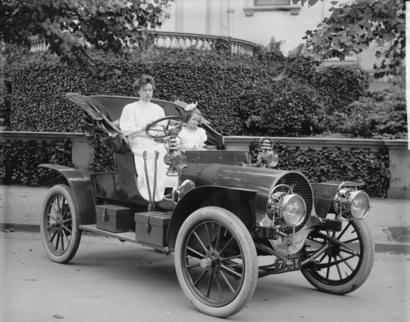
\includegraphics[width=\linewidth]{figures/sample-franklin.png}
    \caption{Description of the figure}
    \label{fig:key-here}
\end{figure}

You should always reference figures in the text, e.g \Cref{fig:key-here}.

\section{Case Study}

\section{Discussion}

\section{Conclusions and Future Works}

\section*{Acknowledgments}

Remove this section if not needed

\bibliography{ceur-article-template}

\end{document}
